\section{API REST}

\subsection{Requisiti}
Per utilizzare le \textit{API REST} non è necessario essere autenticati. Qualsiasi utente può effettuare richieste alle \textit{API} tramite un qualsiasi \textit{client HTTP}.

\subsection{Funzionalità}
Tramite le \textit{API} è possibile ottenere informazioni riguardanti le recensioni e gli utenti. Le richieste possono essere effettuate tramite un qualsiasi \textit{client HTTP}, come ad esempio \texttt{curl} o \texttt{wget}. Le risposte sono in formato \textit{JSON}\glo.

\subsubsection{Recensioni rilasciate e ricevute}
All'indirizzo \path{/reviews/{indirizzo_utente}} è possibile ottenere la lista delle recensioni ricevute da un utente, mentre all'indirizzo \path{/reviews/sender/{indirizzo_utente}} è possibile ottenere la lista delle recensioni inserite.

\begin{figure}[H]
    \centering
    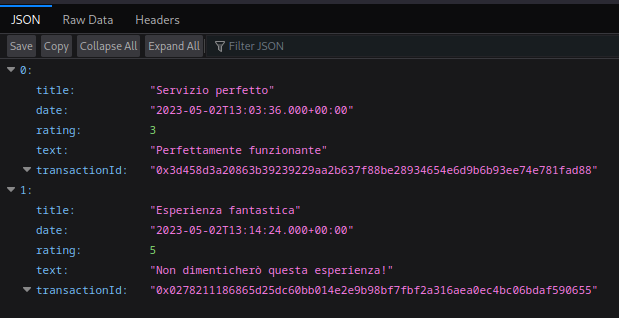
\includegraphics[width=0.6\textwidth]{src/img/api_reviews}
    \caption{Esempio di risposta alla richiesta di recensioni}\label{fig:api_reviews}
\end{figure}

\subsubsection{Dettagli singola recensione}
All'indirizzo \path{/review/{id_recensione}} è possibile ottenere i dettagli di una recensione.

\begin{figure}[H]
    \centering
    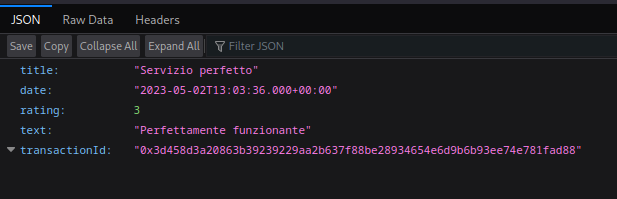
\includegraphics[width=0.6\textwidth]{src/img/api_single_review}
    \caption{Esempio di risposta alla richiesta di dettagli di una recensione}
    \label{fig:api_single_review}
\end{figure}